\documentclass[a4paper,12pt]{article}
\usepackage{graphicx, float, fancyheadings, a4wide, makeidx, verbatim,avant,helvet}
\usepackage{}
\pagestyle{fancyplain}
\setlength{\parindent}{0pt}
\setlength{\parskip}{6pt}

\newcommand{\param}[1] {\textless{}#1\textgreater{}}

\title{\sf{Datasheet for Infra Red Receiver}}
\lfoot{\tiny{\copyright L.P.Klyne}}

\author{Andy Harris}

\makeindex

\begin{document}

\maketitle

\begin{figure}[H]
\centering

\includegraphics[width=0.4\textwidth]{Images/WebBrickSystems.png}
\end{figure}

\begin{figure}[H]
\centering

\includegraphics[width=0.3\textwidth]{Images/wb_logo.jpg}
\end{figure}


\begin{description}
\item[Feb 2007 Document Version 1.00]
\end{description}

\begin{description}
\item[http:\\www.webbricksystems.com] for company information
\item[http:\\www.webbrick.co.uk] for webbrick information
\end{description}

\pagebreak

\section{Infra Red Sensor}
\index{Infra Red Sensor}

\begin{figure}[H]
\centering
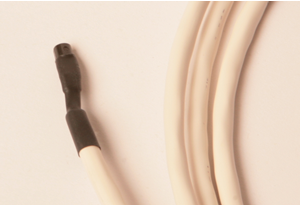
\includegraphics[width=0.4\textwidth]{Images/InfraRedSensorPic.png}
\end{figure}

\subsection{WebBricks and Infra Red Sensors}

The webbrick can receive RC5 infra red signals, these signals can operate the webbrick directly and/or send events that a
WebBrick gateway can respond to. We also supply a simple 8 button remote control that actions sigital inputs 0 to 7. This can be used
for simple local control.


	\begin{itemize}
	  
	  \item{Cable:} Cat 5E cable is recommended for Infra Red sensor connections.  
                    Webbrick Systems supply
	  		Infra Red sensors with 2M Cat 5E pre-attached.
	  		
	  \item{Bus Length:}  We recommend a maximum cable length of 20M ??? for the sensor.
	  			
	  \item{Unused cores:} We recommend that unused cores are connected to ground.  In particular the brown core
	  			should be connected to ground.
	  			
	\end{itemize}

\subsection{Connections}

The following connections should be made:

\begin{figure}[H]
\centering
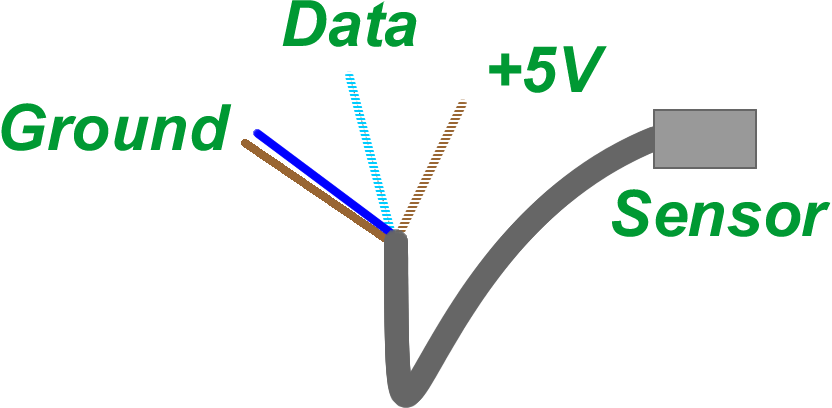
\includegraphics[width=0.6\textwidth]{Images/InfraRedSensorWiring.png}
\end{figure}

	\begin{itemize}
	  
	  \item{Brown-White:} +5V
	  		
	  \item{Blue-White:} Data, this connects to digital input 11, the highest digital input.

	  \item{Blue:} Ground 

	  \item{Brown:} Ground, this core is not connected to the temperature sensor,
	  		grounding this core satisfies the EMC conditions of CE marking.
	  			
	\end{itemize}

Note that multiple Infra Red sensors cannot be connected.

\subsection{Configuration}

Login to the webbrick and access the advanced configuration page. The following page should appear.

\begin{figure}[H]
\centering
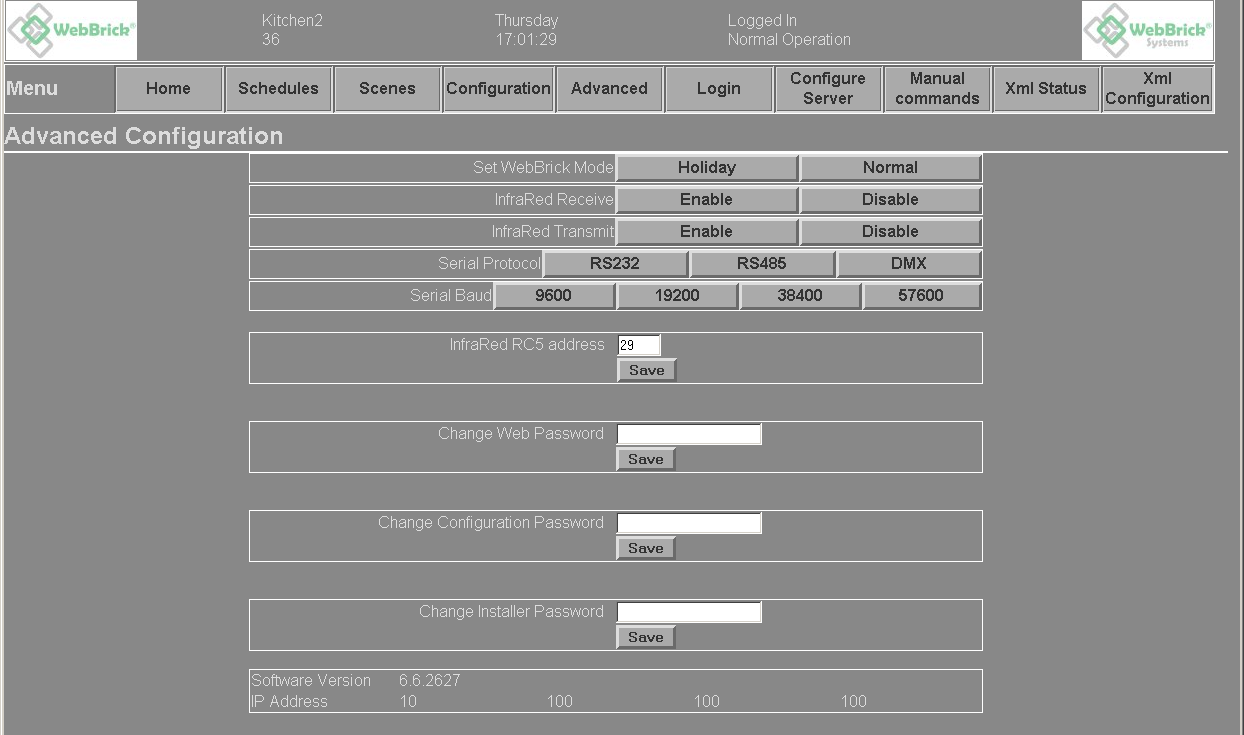
\includegraphics[width=0.6\textwidth]{Images/Advanced.png}
\end{figure}

Click on the Infra Red Receive Enable button. The webbrick will now map the RC5 commands 0-11 on address 29 to the 12 digital inputs. All other 
received RC5 IR commands are sent to the WebBrick Gateway for possible actions. Look in the WebBrick Gateway EventLog for events received.

If you have a different Infra Red controller that sends using a different address then the InfraRed RC5 address can be changed.



\end{document}
